% These are stopped-run diagnostics, not DRL planning performance figures.
\begin{figure}[t]
  \centering
  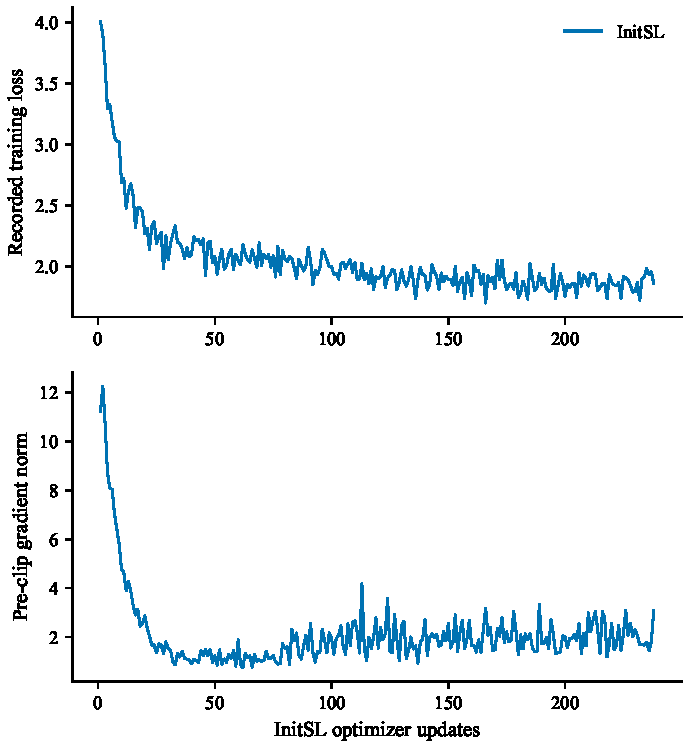
\includegraphics[width=0.48\textwidth]{figures/fig1_training.pdf}
  \caption{Recorded SL initialization loss (mean action NLL per task, then mean over eight tasks) and pre-clipping global gradient norm; the clipping threshold is one for completed updates 1--238. Each point is one actual update without smoothing. Update 239 was not committed after a ledger-persistence exception; SL512 was not reached and the paired DRL stage was not started. These diagnostics do not measure planning improvement.}
  \label{fig:m2_partial_sl_diagnostics}
\end{figure}

\begin{figure}[t]
  \centering
  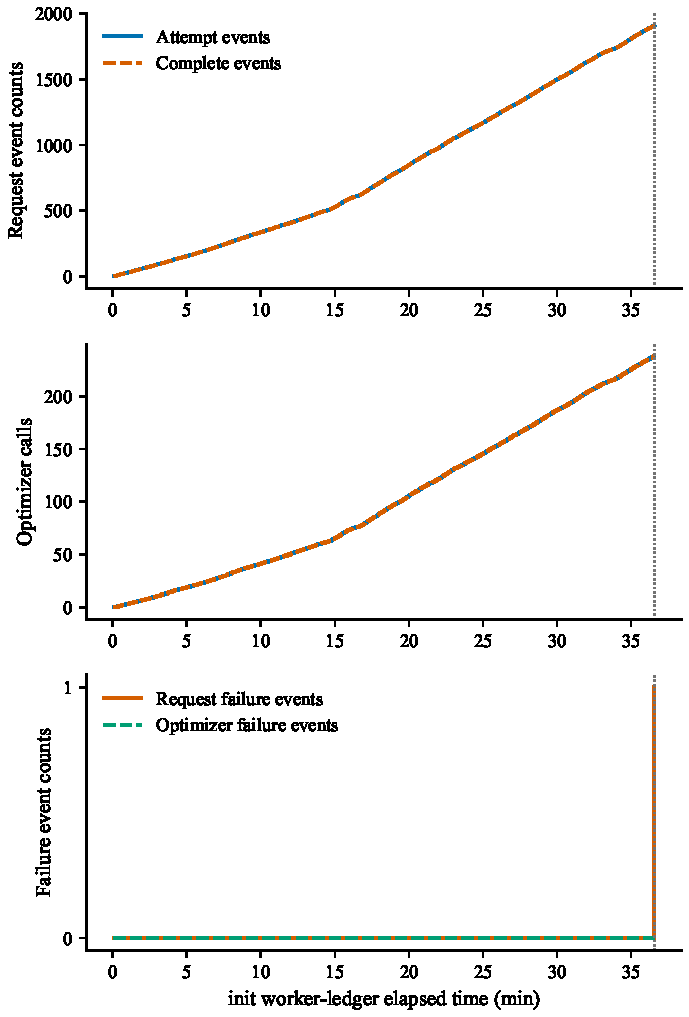
\includegraphics[width=0.48\textwidth]{figures/fig4_resources.pdf}
  \caption{Recorded request, optimizer and failure events over worker-ledger elapsed time. Request complete and failed events are not mutually exclusive: one of the 1910 unique requests has both events, leaving 1909 requests without a failed event. The dotted line marks the recorded failure. The independently measured outer cumulative wall time is 2221.312 seconds and has a different time origin.}
  \label{fig:m2_stopped_resource_events}
\end{figure}

% F2 and F3: NOT_GENERATED. No paired evaluation endpoint ran; missing costs
% and gains must not be plotted as zeros.
